\documentclass{article}

\usepackage{graphicx}
\usepackage{tikz}
\usepackage{tikzsymbols}
\usetikzlibrary{calc,patterns,shapes.geometric}
\pagestyle{empty}
\usepackage[margin=0pt]{geometry}
\geometry{papersize={14in,12in}}

\def\centerarc[#1](#2)(#3:#4:#5){\draw[#1] ($(#2)+({#5*cos(#3)},{#5*sin(#3)})$) arc (#3:#4:#5);}

\begin{document}
	\begin{figure}
		\centering
		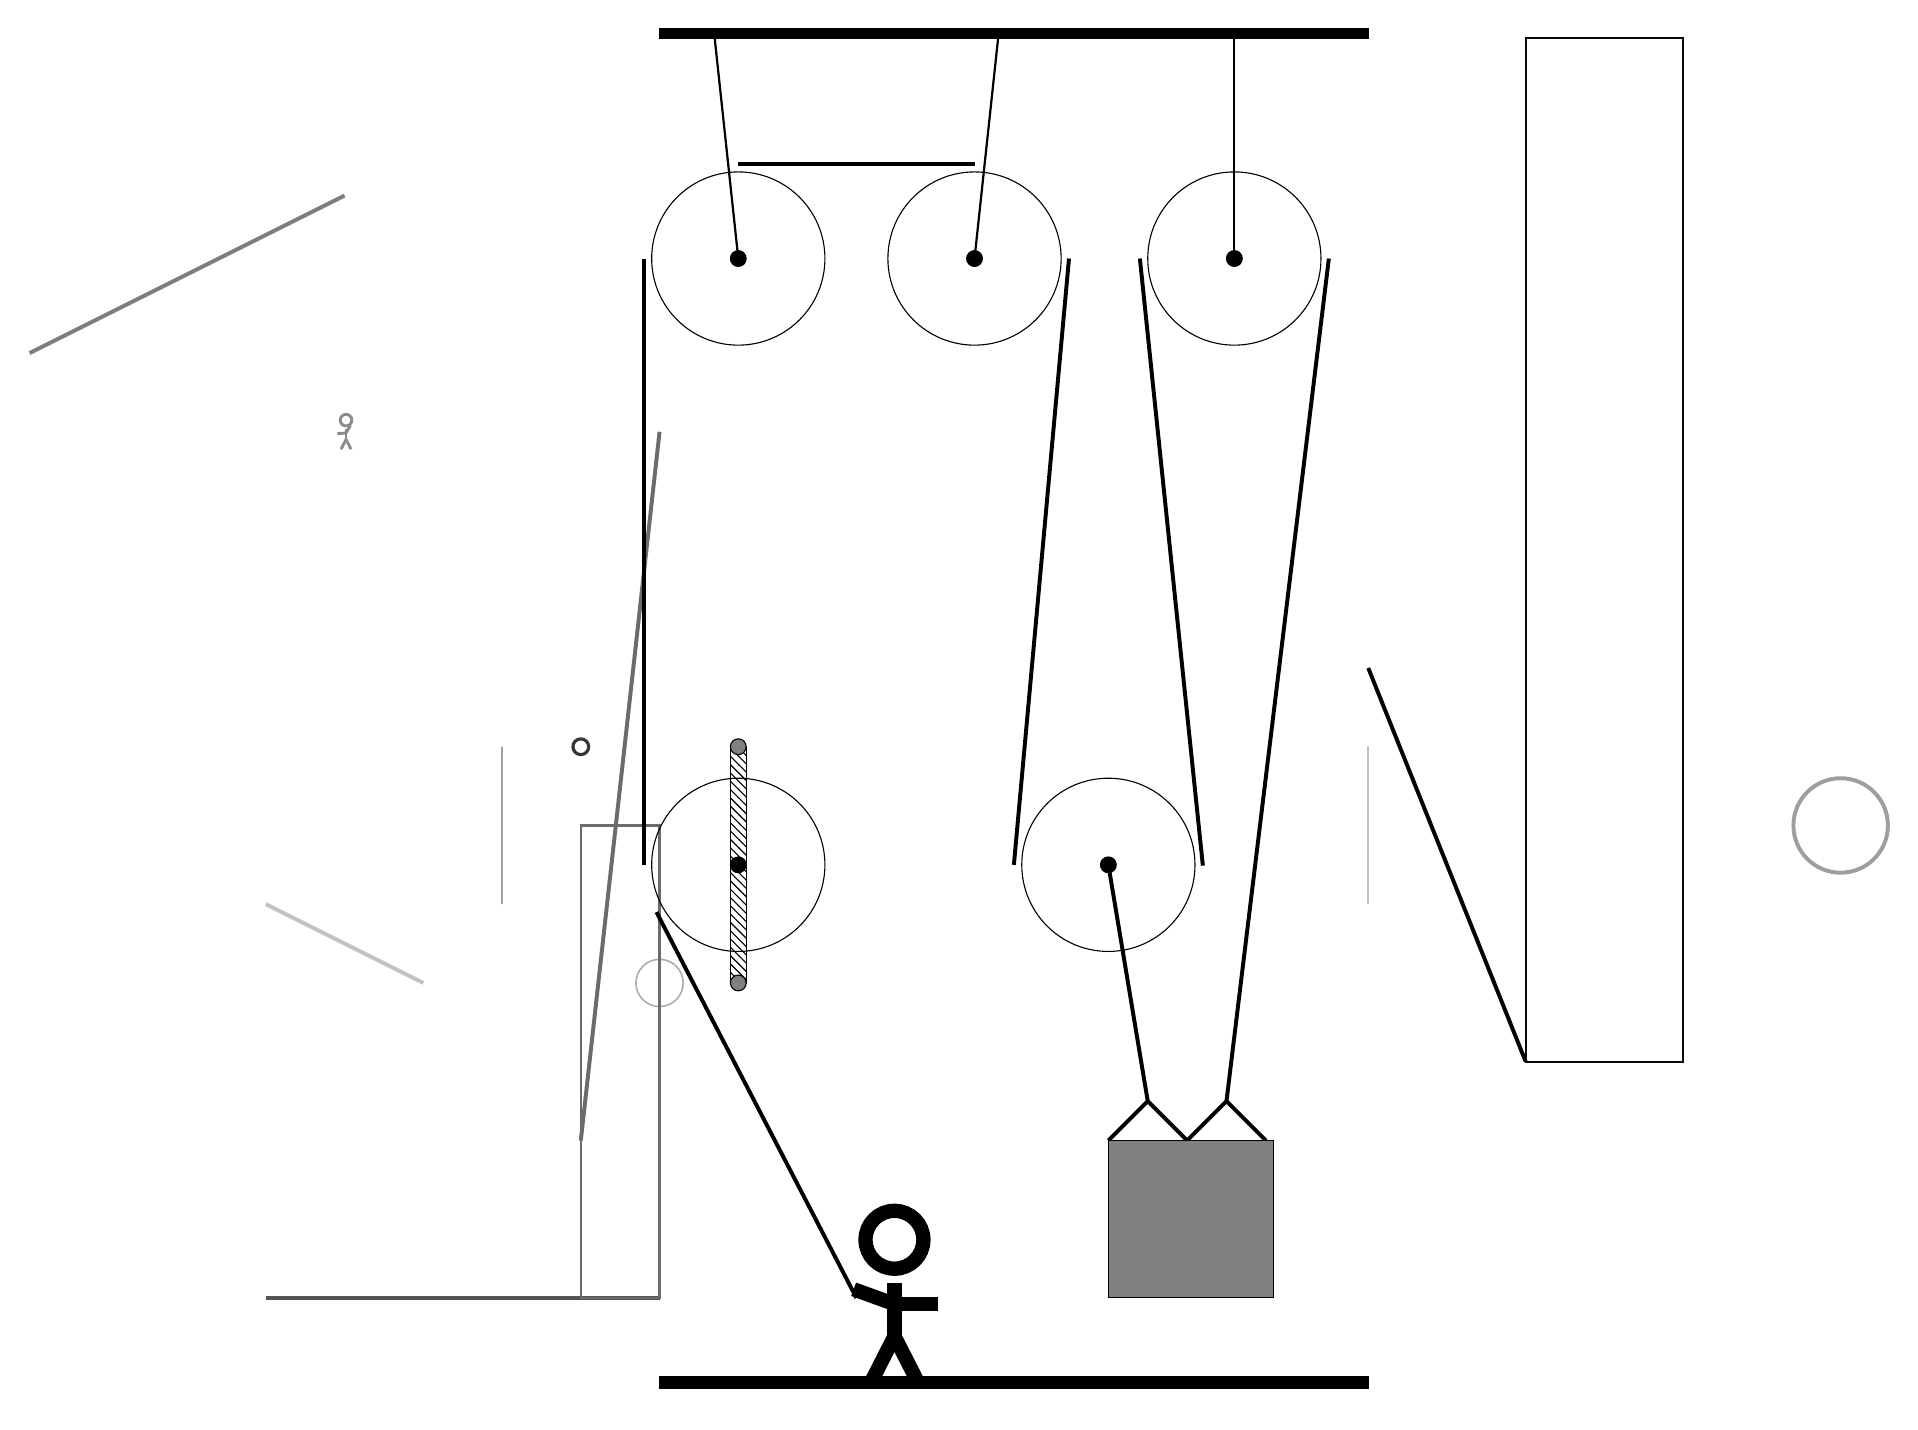
\begin{tikzpicture}
			%%%%% START %%%%%
			
			\draw[fill=black] (-3, 14) rectangle (6, 14.125);
			
			\draw (1, 11.2) circle (1.1);
			\draw[fill=black] (1, 11.2) circle (0.1);
			\draw[thick] (1, 11.2) -- (1.3, 14);
			
			\draw (4.3, 11.2) circle (1.1);
			\draw[fill=black] (4.3, 11.2) circle (0.1);
			\draw[thick] (4.3, 11.2) -- (4.3, 14);
			
			\draw (2.7, 3.5) circle (1.1);
			\draw[fill=black] (2.7, 3.5) circle (0.1);
			
			\draw[line width=0.5mm, color=black!51](-7, 12) -- (-11, 10);
			
			\draw [line width=0.2mm, color=black!33](-3, 2) circle (0.3);
			\draw[line width=0.3mm, color=black!24] (6, 3) rectangle (6, 5);
			\draw[line width=0.5mm, color=black!99](6, 6) -- (8, 1);
			\node[line width=0.6mm, color=black!46] at (-7, 9) {\Strichmaxerl[2][4][60]};
			\draw[line width=0.3mm, color=black!97] (8, 1) rectangle (10, 14);
			\draw [line width=0.5mm, color=black!38](12, 4) circle (0.6);
			
			\draw [line width=0.4mm, color=black!79](-4, 5) circle (0.1);
			\draw[line width=0.5mm, color=black!24](-8, 3) -- (-6, 2);
			\draw[line width=0.5mm, color=black!67](-3, -2) -- (-8, -2);
			\draw[line width=0.5mm, color=black!58](-3, 9) -- (-4, 0);
			\draw[line width=0.3mm, color=black!58] (-3, -2) rectangle (-4, 4);
			\draw[line width=0.3mm, color=black!36] (-5, 3) rectangle (-5, 5);
			
			
			\draw[line width=0.5mm]  (2.7, 0) -- (3.2, 0.5) -- (3.7, 0) -- (4.2, 0.5) -- (4.7, 0);
			\draw[fill=black!50] (2.7, 0) rectangle (4.8, -2);
			
			\draw (-2, 11.2) circle (1.1);
			\draw[fill=black] (-2, 11.2) circle (0.1);
			\draw[thick] (-2, 11.2) -- (-2.3, 14);
			
			\draw (-2, 3.5) circle (1.1);
			\draw[fill=black] (-2, 3.5) circle (0.1);
			\draw[pattern=north west lines, pattern color=black] (-2.1, 5.0) rectangle (-1.9, 2.0);
			\draw[fill=black!50] (-2, 5.0) circle (0.1);
			\draw[fill=black!50] (-2, 2.0) circle (0.1);
			
			\draw[line width=0.5mm](-0.5, -2) -- (-3.0392, 2.9);
			\centerarc[line width=0.5mm](-2, 3.5)(180:210:1.2000000000000002);
			\draw[line width=0.5mm](-3.2, 3.5) -- (-3.2, 11.2);
			\centerarc[line width=0.5mm](-2, 11.2)(90:180:1.2000000000000002);
			
			\draw[line width=0.5mm](-2, 12.4) -- (1, 12.4);
			\centerarc[line width=0.5mm](1, 11.2)(0:90:1.2000000000000002);
			\draw[line width=0.5mm](2.2, 11.2) -- (1.5, 3.5);
			\centerarc[line width=0.5mm](2.7, 3.5)(180:370:1.2000000000000002);
			\draw[line width=0.5mm] (3.9, 3.49) -- (3.1, 11.2);
			\centerarc[line width=0.5mm](4.3, 11.2)(0:180:1.2000000000000002);
			\draw[line width=0.5mm](4.2, 0.5) -- (5.5, 11.2);
			\draw[line width=0.5mm] (3.2, 0.5) -- (2.7, 3.5);
			
			\node at (0, -2) {\Strichmaxerl[10][-20][0]};
			
			\draw[fill=black] (-3, -3) rectangle (6, -3.15);
			
			%%%%% END %%%%%
		\end{tikzpicture}
	\end{figure}	
\end{document}